\let\textcircled=\pgftextcircled
\chapter{Project Outline}
\label{chap:proj_outline}

\section{Description of tasks}

\begin{enumerate}
    \item \textbf{Project environment setup} 
    	\begin{enumerate}
    		\item Download KITTI Dataset
    		\item Split into training and test data
    		\item Install Tensorflow and necessary libraries 
    		\item Review related implementations
    	\end{enumerate}
    \item \textbf{DNN implementation}
   		\begin{enumerate}
   			\item Transform data into valid input
   			\item Develop Voxel Feature Encoding Layer
   			\item Develop CNN for object detection
   			\item Integrate VFE and CNN layers \\ 
   			\textbf{Milestone:}Prototype RPN model 
   			\item Add functionality for object classes 
   			\item RPN Training \\ 
   			\textbf{Milestone -}Publish source code 
   		\end{enumerate}
   	Deliverable: Robust and accurate object detection RPN.
    \item \textbf{Testing and debugging} 
    	\begin{enumerate}
    		\item Initial testing
    		\item Initial debugging
    		\item Test added functionality 
    		\item Debug added functionality 
    	\end{enumerate}
    \item \textbf{Parameter tuning} 
    	\begin{enumerate}
    		\item Compile parameters to test
    		\item Run model with parameters
    		\item Compile results \\ 
    		\textbf{Milestone -} Obtain best performing parameters
    	\end{enumerate}
    \item \textbf{Evaluation} 
    	\begin{enumerate}
    		\item Obtain results of related implementations 
    		\item Run benchmark tests
    		\item Compare results
	    \end{enumerate}
    	  	
    \item \textbf{Validation with different datasets} 
    	\begin{enumerate}
    		\item Download extra datasets 
    		\item Split data into training and test data 
    		\item Transform data into valid input
    		\item Evaluate model performance.
    		
    	\end{enumerate}
    	\textbf{Deliverable -} Performance analysis of model against different datasets.
    
    \item \textbf{Report}
    	\begin{enumerate}
    		\item Write Up system design
    		\item Compile Evaluation results 
    		\item Compile validation results 
    		\item Analyse results 
    		\item Editing and Formatting
    	\end{enumerate}
    \textbf{Deliverable -} Final thesis document. 

	\item \textbf{Poster}
	\begin{enumerate}
		\item Poster design 
		\item Editing and formatting 
	\end{enumerate}
	\textbf{Deliverable - } Final poster
\end{enumerate}



\begin{landscape}
	\section{Timeline and Risk Anaysis }
	\begin{table}[H]
		
		\begin{tabular}{| p{5cm} | l | l | p{5cm} | p{5cm}| }
			\hline
			Risk & Likelihood & Severity & Prevention & Contingency \\ \hline 
			
			Software Library incompatibility & 4 & 2 & Ensure necessary libraries and dependencies are installed beforehand  &  Use of ready instances on cloud platforms.\\  \hline 
			
			Loss of data & 1 & 3 & Frequent backups to GitHub and other local machines. & Datasets can be redownloaded from public websites.  \\ \hline
			
			Overestimated technical capability & 3 & 2 & Review related implementations and literature before beginning project & Large support community for Python and Tensorflow online and within university department. \\ \hline 
			
			Illness or injury & 2 & 3 & Avoid extreme sports and activities & Ensure adequate time has been allocated in timeline to account for unexpected disruptions. \\ \hline 
			
			Long GPU queue on Blue Crystal4 & 4 &3 & Queue work during low peak times & Use cloud instances for training \\ 
			\hline 
			
		\end{tabular}
		\caption{Risk Analysis Table}
		\label{table:risk analysis}
	\end{table}
	
\end{landscape}


\newpage

\begin{landscape}
	\begin{figure}
		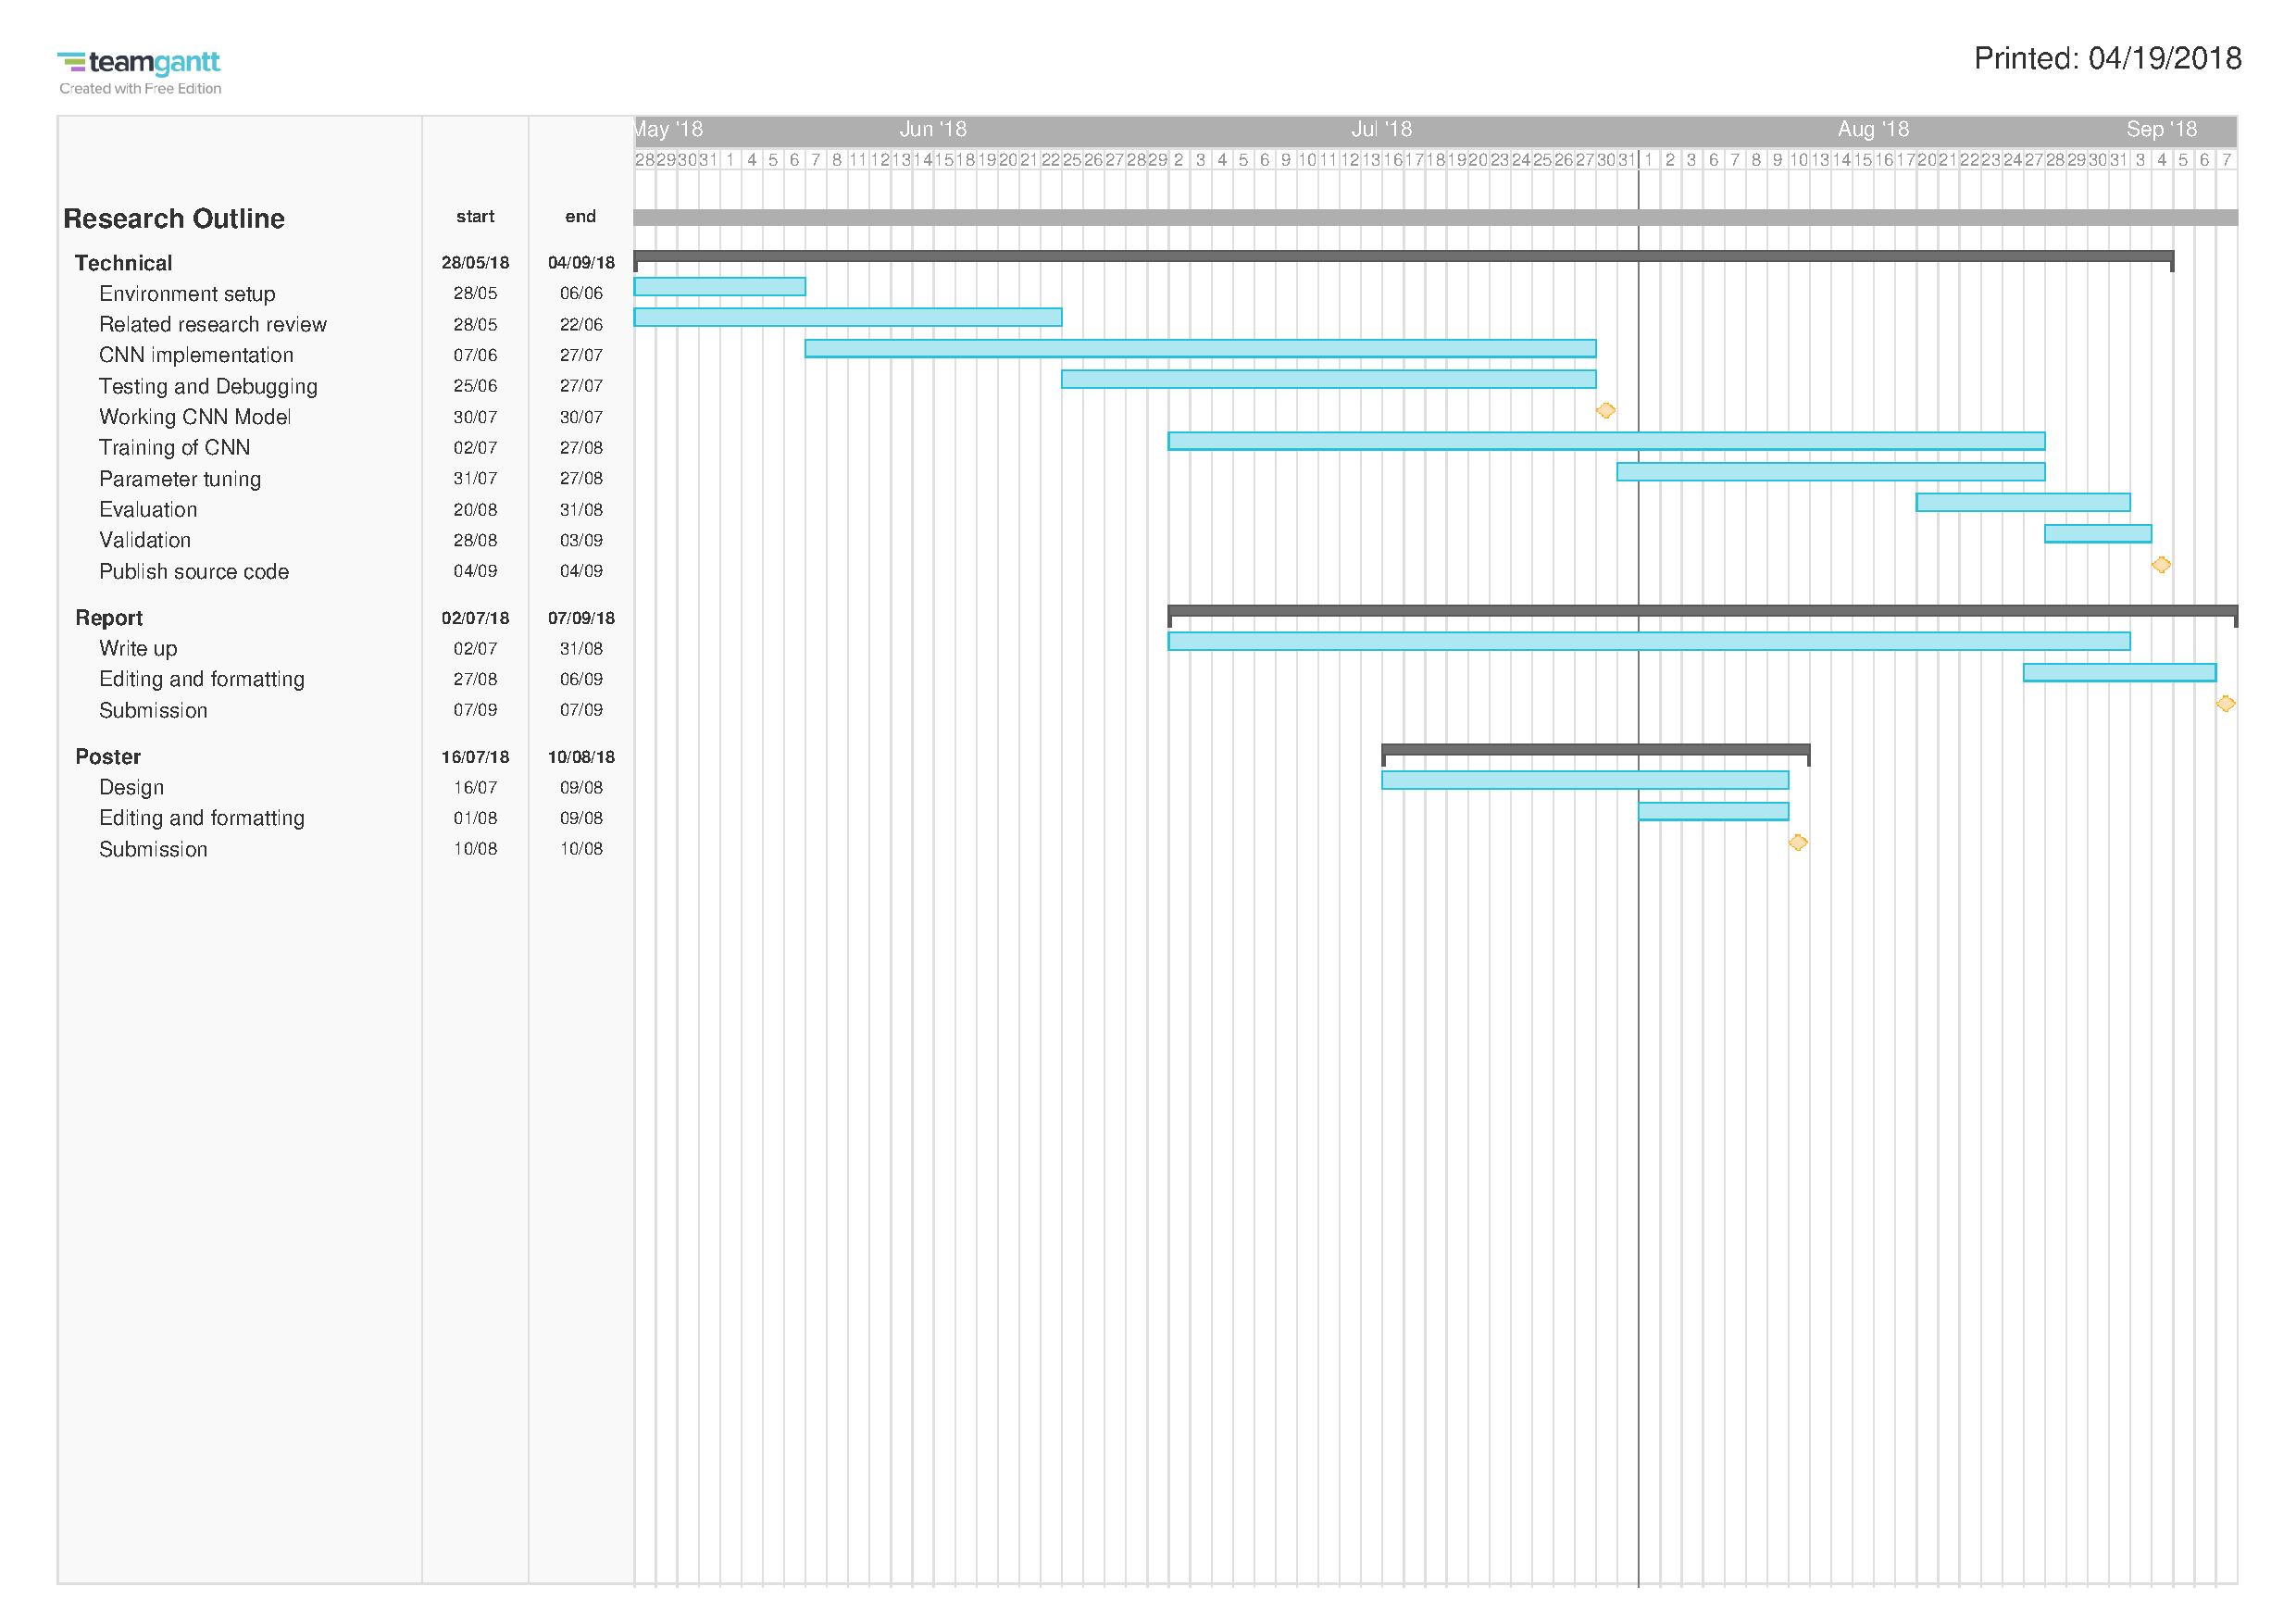
\includepdf[angle=90,scale=0.8]{outline.pdf}
		\caption*{heading}
	\end{figure}
\end{landscape}



